% !TeX program = lualatex
\RequirePackage{iftex}
\ifLuaTeX\else
  \GenericError{}{This document must be compiled with LuaLaTeX.}{}{Run `latexmk -lualatex sample.tex` or set your editor's TeX engine to LuaLaTeX.}
  \expandafter\endinput
\fi
\documentclass[9pt]{beamer}
\usepackage{luatexja}
\usepackage{mathtools}
\usepackage{amssymb}
\usepackage{amsthm}
\usepackage{braket}
\usepackage{bm}
\usepackage{booktabs}
\usepackage{array}
\usepackage{tikz}
\usetikzlibrary{arrows.meta, calc}

\setbeamertemplate{proof begin}{}
\setbeamertemplate{proof end}{}

\usetheme[block=fill]{metropolis}

\setbeamersize{
  text margin left=5mm,
  text margin right=5mm
}

%%%%%%%%%%%%%%%%%%%%%%%%%%%%%%%% １ページ目 %%%%%%%%%%%%%%%%%%%%%%%%%%%%%%%%%
\title{数学講究第３回}
\author{今泉 力}
\date{2026年5月13日}

\begin{document}
\begin{frame}
  \titlepage
\end{frame}

%%%%%%%%%%%%%%%%%%%%%%%%%%%%%%%%% ２ページ目 %%%%%%%%%%%%%%%%%%%%%%%%%%%%%%%%%
\begin{frame}
  \frametitle{第２回の反省}
  \begin{itemize}
    \item テンソル積の性質4
    \item ベル状態の性質について\dots 測定について
  \end{itemize}
\end{frame}

%%%%%%%%%%%%%%%%%%%%%%%%%%%%%%%%%% ３ページ目 %%%%%%%%%%%%%%%%%%%%%%%%%%%%%%%%%
\begin{frame}
  \frametitle{テンソル積の性質4}
  \begin{block}{テンソル積の性質4}
    $\forall \ket{\varphi}, \ket{\psi}, \ket{\chi}, \ket{\omega} \in \mathbb{C}^n$に対して、
    \begin{align}
      \left( \bra{\varphi} \otimes \bra{\psi} \right) \left( \ket{\chi} \otimes \ket{\omega} \right) = \braket{\varphi | \chi} \braket{\psi | \omega}
    \end{align}
  \end{block}
  \begin{proof}
    \textbf{proof.}\\
    インデックスiとjを用いて, $\bra{\varphi}$の$i$成分を$\varphi_i^*$, $\ket{\chi}$の$i$成分を$\chi_i$, $\bra{\psi}$の$j$成分を$\psi_j^*$, $\ket{\omega}$の$j$成分を$\omega_j$とする.
    \begin{align}
      \left( \bra{\varphi} \otimes \bra{\psi} \right)\text{の}(i,j)\text{成分} &= \varphi_i^* \psi_j^* \\
      \left( \ket{\chi} \otimes \ket{\omega} \right)\text{の}(i,j)\text{成分} &= \chi_i \omega_j \\
      \therefore \text{(左辺)} &= \sum_{i,j} \varphi_i^* \psi_j^* \chi_i \omega_j \\
      \text{(右辺)} &= \left( \sum_{i} \varphi_i^* \chi_i \right) \left( \sum_{j} \psi_j^* \omega_j \right) \\
      &= \sum_{i,j} \varphi_i^* \psi_j^* \chi_i \omega_j
    \end{align}
  \end{proof}
\end{frame}

%%%%%%%%%%%%%%%%%%%%%%%%%%%%%%%%%% ４ページ目 %%%%%%%%%%%%%%%%%%%%%%%%%%%%%%%%%
\begin{frame}
  \frametitle{ブロッホ球}
  1量子ビット$\ket{\varphi}$について\begin{align}
    \ket{\varphi} = \alpha \ket{0} + \beta \ket{1}, \quad (|\alpha|^2 + |\beta|^2 = 1)
  \end{align}
  であるとする. ここで, $\alpha$と$\beta$は複素数であるので, 極形式で表す.
  \begin{align}
    \alpha = r_0 e^{i \gamma_0}, \quad \beta = r_1 e^{i \gamma_1} \quad (r_0, r_1 \in \mathbb{R}_{\geq 0}, \gamma_0, \gamma_1 \in \mathbb{R})
  \end{align}
  とする. ($\because$ オイラーの公式)  \\
  $|\alpha|^2 + |\beta|^2 = 1$より、実数パラメータ$\theta$を用いて$r_0 = \cos \left( \frac{\theta}{2} \right)$, $r_1 = \sin \left( \frac{\theta}{2} \right)$とすると
  \begin{align}
    \ket{\varphi} &= \cos \left( \frac{\theta}{2} \right) e^{i \gamma_0} \ket{0} + \sin \left( \frac{\theta}{2} \right) e^{i \gamma_1} \ket{1} \\
    &= e^{i \gamma_0} \left( \cos \left( \frac{\theta}{2} \right) \ket{0} + e^{i (\gamma_1 - \gamma_0)} \sin \left( \frac{\theta}{2} \right) \ket{1} \right)
  \end{align}
\end{frame}

%%%%%%%%%%%%%%%%%%%%%%%%%%%%%%%%%%% ５ページ目 %%%%%%%%%%%%%%%%%%%%%%%%%%%%%%%%%
\begin{frame}
  \frametitle{ブロッホ球}
  \begin{block}{確率振幅}
    $\ket{\varphi} = \alpha \ket{0} + \beta \ket{1}$に対して, $\alpha$と$\beta$を\textbf{確率振幅}と呼ぶ.
    量子状態$\ket{\varphi}$を測定したとき、$\ket{0}$が得られる確率は$|\alpha|^2$であり、$\ket{1}$が得られる確率は$|\beta|^2$である.
  \end{block}
  \begin{block}{グローバル位相}
    任意の量子状態$\ket{\varphi}$と$|z| = 1$を満たす複素数$z$に対して, $z \ket{\varphi}$は$\ket{\varphi}$と同じ意味を持つ.
    $z$を$\ket{\varphi}$の\textbf{グローバル位相}と呼ぶ.
  \end{block}
  $\ket{\varphi} = \alpha \ket{0} + \beta \ket{1}$とする. $z$を$|z| = 1$を満たす複素数とすると, 
  \begin{align}
    z \ket{\varphi} = z \alpha \ket{0} + z \beta \ket{1}
  \end{align}
  なので, $z \ket{\varphi}$が得られる確率は$|z \alpha|^2 = |\alpha|^2$, $\ket{1}$が得られる確率は$|z \beta|^2 = |\beta|^2$であり, $\ket{\varphi}$と同じ確立である.
\end{frame}

%%%%%%%%%%%%%%%%%%%%%%%%%%%%%%%%%%%% ６ページ目 %%%%%%%%%%%%%%%%%%%%%%%%%%%%%%%%%
\begin{frame}
  \frametitle{ブロッホ球}
  式(10).について, グローバル位相である$e^{i \gamma_0}$を無視し, $\gamma_1 - \gamma_0 = \phi$とすると
  \begin{align}
    \ket{\varphi} = \cos \left( \frac{\theta}{2} \right) \ket{0} + e^{i \phi} \sin \left( \frac{\theta}{2} \right) \ket{1} \quad \big( \theta \in [0, \pi], \phi \in [0, 2\pi) \big)
  \end{align}
  よって, 量子状態$\ket{\varphi}$は実数パラメータ$\theta$と$\phi$を用いて, \textbf{ブロッホ球}上の点として表すことができる.
  \begin{center}
  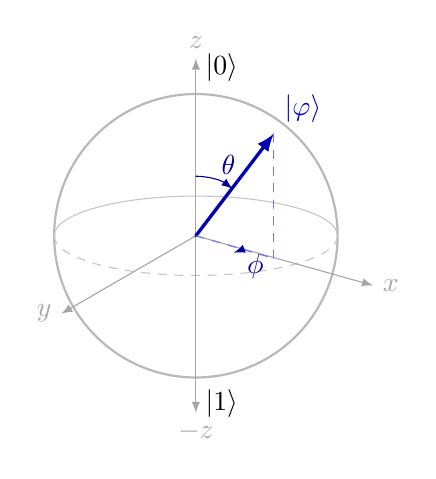
\begin{tikzpicture}[
  scale=1.8,
  line cap=round,
  line join=round,
  >=latex
]
  % ===== theta と phi を調整する場所 =====
  % 状態ベクトル |varphi> の先端です。
  % theta や phi を大きく変えるときは、この点も一緒に動かします。
  \coordinate (varphi) at (0.55,0.72);

  % 状態ベクトルを赤道面に下ろした点です。
  % phi を変えるときは、この点を赤道上で左右に動かします。
  \coordinate (varphiProjection) at (0.55,-0.16);

  % theta の弧の終点角度です。
  % 90度が z軸方向で、値を小さくすると |varphi> が右側へ倒れます。
  \def\ThetaEndAngle{52}

  % phi の弧の始点・終点角度です。
  % 今は -16度から -37度まで描いています。
  % phi を大きく見せたいときは \PhiEndAngle をさらに小さくします。
  \def\PhiStartAngle{-16}
  \def\PhiEndAngle{-37}

  % 球体
  \draw[gray!55, thick] (0,0) circle (1);
  \draw[gray!45, dashed] (-1,0) arc[start angle=180, end angle=360, x radius=1, y radius=0.28];
  \draw[gray!45] (1,0) arc[start angle=0, end angle=180, x radius=1, y radius=0.28];

  % 座標軸
  \draw[->, gray!70] (0,0) -- (0,1.25) node[above] {$z$};
  \draw[->, gray!70] (0,0) -- (0,-1.25) node[below] {$-z$};
  \draw[->, gray!70] (0,0) -- (1.25,-0.35) node[right] {$x$};
  \draw[->, gray!70] (0,0) -- (-0.95,-0.55) node[left] {$y$};

  % 基底状態
  \node[above right] at (0,1.02) {$\ket{0}$};
  \node[below right] at (0,-1.02) {$\ket{1}$};

  % 量子状態
  \draw[very thick, blue!70!black, ->] (0,0) -- (varphi) node[above right] {$\ket{\varphi}$};

  % 点線
  \draw[blue!55, dashed] (varphi) -- (varphiProjection);
  \draw[blue!55, dashed] (0,0) -- (varphiProjection);

  % 角度
  \draw[->, blue!60!black] (0,0.42) arc[start angle=90, end angle=\ThetaEndAngle, radius=0.42];
  \node[blue!60!black] at (0.23,0.50) {$\theta$};

  \draw[->, blue!60!black] (0.32,-0.09) arc[start angle=\PhiStartAngle, end angle=\PhiEndAngle, x radius=0.32, y radius=0.09];
  \node[blue!60!black] at (0.42,-0.22) {$\phi$};
\end{tikzpicture}

  \end{center}
\end{frame}

%%%%%%%%%%%%%%%%%%%%%%%%%%%%%%%%%%%%% ７ページ目 %%%%%%%%%%%%%%%%%%%%%%%%%%%%%%%%%
\begin{frame}
  \frametitle{アダマール基底}
  $\phi$回転（Y軸周りの回転）を行う行列と, $R_y(\phi)$と$\theta$回転（Z軸周りの回転）を行う行列$R_z(\theta)$は以下のようにあらわすことができる.
  \begin{align}
    R_y(\phi) \coloneq \begin{bmatrix}
      \cos \left( \frac{\phi}{2} \right) & -\sin \left( \frac{\phi}{2} \right) \\
      \sin \left( \frac{\phi}{2} \right) & \cos \left( \frac{\phi}{2} \right)
    \end{bmatrix}, \quad
    R_z(\theta) \coloneq \begin{bmatrix}
      e^{-i\frac{\theta}{2}} & 0 \\
      0 & e^{i\frac{\theta}{2}}
    \end{bmatrix}
  \end{align}
  ここで, $\phi = \frac{\pi}{2}$, $\theta = \pi$とすると
  \begin{align}
    R_y \left( \frac{\pi}{2} \right) R_z(\pi) &= \begin{bmatrix}
      \cos \left( \frac{\pi}{4} \right) & -\sin \left( \frac{\pi}{4} \right) \\
      \sin \left( \frac{\pi}{4} \right) & \cos \left( \frac{\pi}{4} \right)
      \end{bmatrix}
      \begin{bmatrix}
      e^{-i\frac{\pi}{2}} & 0 \\
      0 & e^{i\frac{\pi}{2}}
    \end{bmatrix} \\
    &= \begin{bmatrix}
      \frac{1}{\sqrt{2}} & -\frac{1}{\sqrt{2}} \\
      \frac{1}{\sqrt{2}} & \frac{1}{\sqrt{2}}
    \end{bmatrix}
    \begin{bmatrix}
      -i & 0 \\
      0 & i
    \end{bmatrix}
    = \begin{bmatrix}
      -\frac{i}{\sqrt{2}} & -\frac{i}{\sqrt{2}} \\
      -\frac{i}{\sqrt{2}} & \frac{i}{\sqrt{2}}
    \end{bmatrix} \\
    &= -i \begin{bmatrix}
      \frac{1}{\sqrt{2}} & \frac{1}{\sqrt{2}} \\
      \frac{1}{\sqrt{2}} & -\frac{1}{\sqrt{2}}
    \end{bmatrix}
    \eqqcolon -i H
    \end{align}
    Hは\textbf{アダマール行列}と呼ばれる. $-i$をグローバル位相として無視すると, $H$はX軸とZ軸を入れ替える行列であることがわかる.

\end{frame}

%%%%%%%%%%%%%%%%%%%%%%%%%%%%%%%%%%%%% ８ページ目 %%%%%%%%%%%%%%%%%%%%%%%%%%%%%%%%%
\begin{frame}
  \frametitle{アダマール基底}
  アダマール行列$H$を用いて, $\ket{0}$と$\ket{1}$を以下のように変換することができる.
  \begin{align}
    H \ket{0} = \frac{1}{\sqrt{2}} \left( \ket{0} + \ket{1} \right), \quad
    H \ket{1} = \frac{1}{\sqrt{2}} \left( \ket{0} - \ket{1} \right)
  \end{align}
  \begin{center}
    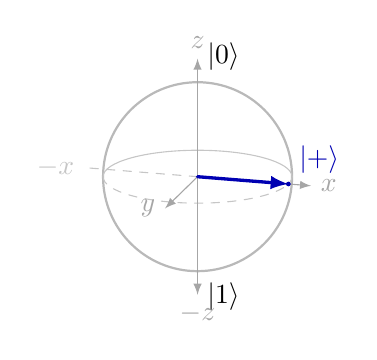
\begin{tikzpicture}[
  scale=1.2,
  line cap=round,
  line join=round,
  >=latex
]
  \tikzset{declare function={view=-16; theta=90; phi=0;}}

  \draw[gray!55, thick] (0,0) circle (1);
  \draw[gray!45, dashed] (-1,0) arc[start angle=180, end angle=360, x radius=1, y radius=0.28];
  \draw[gray!45] (1,0) arc[start angle=0, end angle=180, x radius=1, y radius=0.28];

  \draw[->, gray!70] (0,0) -- (0,1.25) node[above] {$z$};
  \draw[->, gray!70] (0,0) -- (0,-1.25) node[below] {$-z$};
  \draw[->, gray!70] (0,0) -- ({1.25*cos(view)}, {0.28*1.25*sin(view)}) node[right] {$x$};
  \draw[gray!45, dashed] (0,0) -- ({-1.25*cos(view)}, {-0.28*1.25*sin(view)}) node[left] {$-x$};
  \draw[->, gray!70] (0,0) -- ({1.25*cos(view-90)}, {0.28*1.25*sin(view-90)}) node[left] {$y$};

  \node[above right] at (0,1.02) {$\ket{0}$};
  \node[below right] at (0,-1.02) {$\ket{1}$};

  \coordinate (stateProjection) at ({sin(theta)*cos(view-phi)}, {0.28*sin(theta)*sin(view-phi)});
  \coordinate (state) at ({sin(theta)*cos(view-phi)}, {cos(theta) + 0.28*sin(theta)*sin(view-phi)});
  \draw[very thick, blue!70!black, ->] (0,0) -- (state) node[above right] {$\ket{+}$};
  \fill[blue!70!black] (state) circle (0.025);
\end{tikzpicture}

    \hspace{1.2cm}
    \input{figures/figure_-.tex}
  \end{center}
  $\ket{+} \coloneq \frac{1}{\sqrt{2}} \left( \ket{0} + \ket{1} \right)$と$\ket{-} \coloneq \frac{1}{\sqrt{2}} \left( \ket{0} - \ket{1} \right)$を\textbf{アダマール基底}と呼ぶ.
\end{frame}

%%%%%%%%%%%%%%%%%%%%%%%%%%%%%%%%%%%%% ９ページ目 %%%%%%%%%%%%%%%%%%%%%%%%%%%%%%%%%
\begin{frame}
  \frametitle{測定}
  ブロッホ球におけるZ軸の値を読む測定を\textbf{Z測定}という.
  \begin{itemize}
    \item $\ket{0}$はZ測定すると$+1$
    \item $\ket{1}$はZ測定すると$-1$
    \item $\ket{+}$はZ測定すると$0$（？）
  \end{itemize}
  ブロッホ球におけるX軸の値を読む測定を\textbf{X測定}という.
  \begin{itemize}
    \item $\ket{+}$はX測定すると$+1$
    \item $\ket{-}$はX測定すると$-1$
    \item $\ket{0}$はX測定すると$0$（？？）
  \end{itemize}
\end{frame}

%%%%%%%%%%%%%%%%%%%%%%%%%%%%%%%%%%%%% １０ページ目 %%%%%%%%%%%%%%%%%%%%%%%%%%%%%%%%%
\begin{frame}
  \frametitle{測定}
  \begin{itemize}
  \item 量子状態は, 測定すると$\bf{\ket{0}}$\textbf{と}$\bf{\ket{1}}$\textbf{のいずれかになってしまう.} これは経験的事実であり\textbf{ボルンの確率規則}と呼ばれる.
  \item 例えば$\ket{+}$をZ測定すると$+1$になるときもあれば, $-1$になることもある. その確率は$\dfrac{1}{2}$である.
  \item よって量子コンピュータでは, 測定として\textbf{期待値}を計算する.
  \end{itemize}
  $\ket{\varphi} = \alpha \ket{0} + \beta \ket{1}$とする. このとき, Z測定の期待値は
  \begin{align}
    (+1)|\alpha|^2 + (-1)|\beta|^2 = |\alpha|^2 - |\beta|^2
  \end{align}
  $\ket{\varphi}$をアダマール基底を用いて表すと以下のように変換できる
  \begin{align}
    \ket{\varphi} = \alpha \ket{0} + \beta \ket{1} = \frac{\alpha + \beta}{\sqrt{2}} \ket{+} + \frac{\alpha - \beta}{\sqrt{2}} \ket{-}
  \end{align}
  よってX測定の期待値は
  \begin{align}
    (+1)\left| \frac{\alpha + \beta}{\sqrt{2}} \right|^2 + (-1)\left| \frac{\alpha - \beta}{\sqrt{2}} \right|^2 &= \frac{1}{2}(\alpha + \beta)(\alpha^* + \beta^*) - \frac{1}{2}(\alpha - \beta)(\alpha^* - \beta^*)\\
    &= \alpha\beta^* + \alpha^*\beta
  \end{align}
\end{frame}

%%%%%%%%%%%%%%%%%%%%%%%%%%%%%%%%%%%%% １１ページ目 %%%%%%%%%%%%%%%%%%%%%%%%%%%%%%%%%
\begin{frame}
  \frametitle{測定}
  これらの期待値は,ゲート操作である行列を用いて簡単に表現することができる.
  \begin{align}
    \text{（Z測定の期待値）} &= |\alpha|^2 - |\beta|^2\\
    &= \begin{bmatrix} \alpha^* & \beta^* \end{bmatrix} \begin{bmatrix} 1 & 0 \\ 0 & -1 \end{bmatrix} \begin{bmatrix} \alpha \\ \beta \end{bmatrix} = \bra{\varphi}Z\ket{\varphi} \\
    \text{（X測定の期待値）} &= \alpha \beta^* + \alpha^*\beta \\
    &= \begin{bmatrix} \alpha^* & \beta^* \end{bmatrix} \begin{bmatrix} 0 & 1 \\ 1 & 0 \end{bmatrix} \begin{bmatrix} \alpha \\ \beta \end{bmatrix} = \bra{\varphi}X\ket{\varphi}
  \end{align}
  \begin{itemize}
    \item ブラケットで行列を挟むことで, 期待値を計算することができる.
    \item 「ゲート操作である行列」と書いたが, ゲートと測定で扱う行列は別物.
    \item Z測定やX測定のほかにもエルミート行列を用いた測定が存在する.
    \item 測定で扱うエルミート行列を\textbf{観測量}や\textbf{オブザーバブル}という.
  \end{itemize}
\end{frame}

%%%%%%%%%%%%%%%%%%%%%%%%%%%%%%%%%%%%% １２ページ目 %%%%%%%%%%%%%%%%%%%%%%%%%%%%%%%%%
\begin{frame}
  \frametitle{測定}
  ＜なぜ$\bra{\varphi}A\ket{\varphi}$が期待値になるのか＞\\
  \textbf{proof.} \\
  観測量$A \in Mat_{2^n}(\mathbb{C})$はエルミート行列（正規行列）であるので, 実数の固有値$\lambda_i$と, 固有ベクトル$\ket{v_i}$によりスペクトル分解できる. \\
  任意の$i \in \mathbb{N}_{1\le i \le 2^n}$に対し,
  \begin{align}
    A\ket{v_i} = \lambda_i \ket{v_i}
  \end{align}
  また$\ket{v_i}$は直交するので, 任意の量子状態$\ket{\varphi}$に対して$c_i \in \mathbb{C}$が存在し
  \begin{align}
    \ket{\varphi} = \sum_{i \in \mathbb{N}_{1 \le i \le 2^n}} c_i \ket{v_i}
  \end{align}
  ボルンの確率規則により, 測定値$\lambda_i$となる確率は$P\left(\lambda_i\right)$は
  \begin{align}
    P\left( \lambda_i \right) = |c_i|^2
  \end{align}
  よって古典的な定義に従うと, 期待値は$E$は
  \begin{align}
    E = \sum_{i \in \mathbb{N}_{1 \le i \le 2^n}} \lambda_i |c_i|^2
  \end{align}
\end{frame}

%%%%%%%%%%%%%%%%%%%%%%%%%%%%%%%%%%%%% １３ページ目 %%%%%%%%%%%%%%%%%%%%%%%%%%%%%%%%%
\begin{frame}
\frametitle{測定}
$\bra{\varphi}A\ket{\varphi}$を計算する.
\begin{align}
  A\ket{\varphi} &= A \left( \sum_{i \in \mathbb{N}_{1 \le i \le 2^n}} c_i \ket{v_i} \right)\\
  &= \sum_{i \in \mathbb{N}_{1 \le i \le 2^n}} c_i \left( A \ket{v_i} \right) = \sum_{i \in \mathbb{N}_{1 \le i \le 2^n}} c_i \left( \lambda_i \ket{v_i} \right)
\end{align}
また, $\bra{\varphi} = sum_{j \in \mathbb{N}_{1 \le j \le 2^n}}$なので

\end{frame}

\end{document}
